%!TEX root = ../main.tex
Στο δεύτερο κεφάλαιο έχει γίνει μία αναλυτική παρουσίαση των εργαλείων βελτιστοποίησης που παρέχει το Vivado HLS. Στο παρόν κεφάλαιο, θα αναφερθούμε στην προσπάθεια εφαρμογής τους στο πρόγραμμα που αναπτύχθηκε με στόχο τη μείωση της καθυστέρησης. Θα παρουσιαστούν, επίσης, και τα αποτέλεσματα του συστήματος που αναπτύχθηκε.
\section{Βελτιστοποίηση}

Μην έχοντας θέσει συγκεκριμένες προδιαγραφές για το σύστημα, θα προσπαθήσουμε να βρούμε μία μέση λύση ανάμεσα στη μείωση της συνολικής καθυστέρησης και την αξιοποίηση των πόρων. Στόχος μας είναι, επομένως να εντοπίσουμε πιθανές μεθόδους βελτιστοποίησης που θα μας δώσουν τα καλύτερα δυνατά αποτελέσματα.

Πρώτο βήμα κατά τη διαδικασία βελτιστοποίησης είναι η συγγραφή του κώδικα χωρίς κανένα είδος βελτιστοποίησης ώστε να ληφθεί μία baseline μέτρηση με την οποία θα συγκριθούν οι διάφορες βελτιστοποιημένες υλοποιήσεις.

Στη συνέχεια θα εφαρμοστούν διάφοροι συνδυασμοί βελτιστοποιήσεων και θα επιλεχθεί εκείνος που παρέχει την καλύτερη επιτάχυνση και αξιοποίηση πόρων. Στην περίπτωση που κάποιος συνδυασμός οδηγήσει σε κατανάλωση περισσότερων φυσικών πόρων από τους διαθέσιμους της συσκευής, τότε αυτός απορρίπτεται απευθείας. Προσοχή πρέπει να δοθεί στο ότι οι πόροι του συνολικού συστήματος θα αυξηθούν κατά κάποιο ποσοστό όταν θα σχεδιάσουμε το πλήρες σύστημα στο Vivado λόγω της εισαγωγής των περιφερειακών που θα χρησιμοποιηθούν.

Υπάρχουν δύο τρόποι για την εφαρμογή βελτιστοποιήσεων στο Vivado HLS: απευθείας στον πηγαίο κώδικα η σε ξεχωριστό tcl αρχείο. Με το ξεχωριστό αρχείο tcl, διευκολύνεται σε μεγάλο βαθμό η διαδικασία εύρεσης του καλύτερου συνδυασμού καθώς μπορούμε να δημιουργήσουμε πολλαπλά solutions και να εφαρμόσουμε τις βελτιώσεις που περιέχονται στο αρχείο \textbf{directives.tcl} στο καθένα. Και στις δύο περιπτώσεις οι βελτιστοποιήσεις πραγματοποιούνται με τη βοήθεια της ντιρεκτίβας \textbf{\#pragma HLS}.

Ο συνδυασμός βελτιώσεων που παρουσίασε τα καλύτερα αποτελέσματα περιγράφεται στη συνέχεια. Προέκυψε μετά από ένα πλήθος διαφορετικών συνδυασμών / προσεγγίσεων και προσπαθειών. Στην επόμενη ενότητα θα παρατεθούν τα τελικά αποτελέσματα καθώς και μερικές ενδιάμεσες προσπάθειες - τόσο επιτυχημένες όσο και αποτυχημένες.
\subsection{Top συνάρτηση}

Στην κύρια συνάρτηση πραγματοποιούνται 2 βρόχοι για την είσοδο και έξοδο δεδομένων από και προς τον ελεγκτή DΜΑ αντίστοιχα καθώς και οι κλήσεις των συναρτήσεων.

Λόγω της φύσης του αλγορίθμου μας και του τρόπου προσέγγισής μας τα δεδομένα εισόδου έχουν αποθηκευτεί σε BRAM. Οι βρόχοι επομένως που επεξεργάζονται τα δεδομένα απαιτούν την ανάγνωση από την RAM με αποτέλεσμα να εισάγεται καθυστέρηση λόγω του μικρού αριθμού θυρών της. Για το λόγο αυτό επιλέχθηκε να διαρεθούν οι buffers σε μικρότερους ώστε να επιτευχθεί ταχύτερη ανάγνωση και επεξεργασία δεδομένων καθώς και αυξημένη ρυθμοαπόδοσης. Μετά από πολλούς διαφορετικούς συνδυασμούς καταλήξαμε στην καλύτερη δύνατη διαίρεση. Αυτή επιτυγχάνεται με τη ντιρεκτίβα \textbf{array\_partition}.

Πιο συγκεκριμένα, ο μονοδιάστατος πίνακας \textbf{input} διαιρέθηκε κυκλικά, δημιουργώντας έτσι μικρότερους πίνακες μέσω της τεχνικής interleaving \footnote{https://en.wikipedia.org/wiki/Interleaved\_memory}. Πρακτικά, κάθε στοιχείο του πίνακα τοποθετείται σε έναν νέο πίνακα μέχρι να πραγματοποιηθεί η πλήρης διαίρεση. Για παράδειγμα, αν επιλεχθεί ένας βαθμός διαίρεσης, $factor =3$ η διαίρεση θα γίνει ως εξής:
\begin{align*}
input[0] \longrightarrow input1[0] \\
input[1] \longrightarrow input2[0] \\
input[2] \longrightarrow input3[0] \\
input[3] \longrightarrow input4[0]
\end{align*}

Ο καλύτερος συμβιβασμός μεταξύ απόδοσης και κατανάλωσης πόρων επιτεύχθηκε με την κυκλική διαίρεση μόνο στον πίνακα input βαθμού διαίρεσης ίσου με 2 λόγω των πολλαπλών προσπελάσεων του στη συνάρτηση όπου εκτελείται η πράξη της συνέλιξης.

\begin{lstlisting}[language=C++,belowskip=-0.3\baselineskip]
static uint8_t input[IMAGE_WIDTH*IMAGE_HEIGHT];
#pragma HLS array_partition variable=input cyclic factor=2
\end{lstlisting}

\subsection{Γκαουσιανό φίλτρο}

Η συγκεκριμένη συνάρτηση αποτελεί τη πιο "χρονοβόρα" συνάρτηση του αλγορίθμου μας, καθώς περιέχει μαθηματικές πράξεις με floating point μεταβλητές. Αρχικά, με τη χρήση της προηγούμενης βελτίωση που πραγματοποιήθηκε (array cyclic partitioning) μειώθηκε δραστικά ο συνολικός αριθμός κύκλων που απαιτείται για την επεξεργασία των δεδομένων. Εφαρμόστηκε επίσης παραλληλοποίηση στο βρόχο που προσπελαύνει τις στήλες της εικόνας καθώς και στον εσωτερικό βρόχο που διατρέχει τον πυρήνα μετασχηματισμού.

Η βελτιστοποίηση αυτή επέφερε μία δραματική μείωση στους κύκλους ρολογιού καθώς και στο latency της. Πριν τη βελτιστοποίηση, το υλικό που δημιουργήθηκε από το HLS δε θα ήταν εφικτό να επιτύχει στην προσομοίωση λόγω της μεγάλης συχνότητας ρολογιού.

\subsection{grad}

Στη συνάρτηση αυτή εφαρμόσθηκαν εν μέρει αντίστοιχες βελτιώσεις με τις προηγούμενες. Πραγματοποιήθηκε παραλληλοποίηση στους δύο εξωτερικού βρόχους της συνάρτησης καθώς και στον εσωτερικό βρόχο της δεύτερης λειτουργίας της που είναι η εύρεση του μέτρου της κλίσης.

\begin{lstlisting}[language=C++,belowskip=-0.3\baselineskip]
for (i = 0; i < IMAGE_HEIGHT; ++i)
	#pragma HLS pipeline
	for (j = 1; j < IMAGE_WIDTH - 1; ++j)
		find gradX;

for (j = 0; j < IMAGE_WIDTH; ++j)
	#pragma HLS pipeline
	for (i = 1; i < IMAGE_HEIGHT - 1; ++i)
		find gradY;

for (i = 0; i < IMAGE_HEIGHT; ++i)
	for (j = 0; j < IMAGE_WIDTH; ++j, ++t)
		#pragma HLS pipeline
		find gradMag;
\end{lstlisting}
\subsection{edgeID}

Η τεχνική που έδωσε τα καλύτερα αποτελέσματα και σε αυτή την συνάρτηση είναι η παραλληλοποίηση του εσωτερικού βρόχου της συνάρτησης.

\section{Αποτελέσματα}

Για την αξιολόγηση της σωστής λειτουργίας της υλοποίησης μας, συγκρίνονται οπτικά οι εικόνες εξόδου. Επίσης, γίνεται αξιολόγηση των αναγνωρισμένων ακμών για διάφορες τιμές του κατωφλίου. Στην παρούσα ενότητα αναλύονται και τα αποτελέσματα χρονισμού και κατανάλωσης πόρων τόσο στο Vivado HLS όσο και στο Vivado IPI.
\subsection{Αποτελέσματα υλοποίησης}

Αρχικά, παρατίθενται οι μετρήσεις της baseline υλοποίησης. Με βάση αυτές συγκρίνονται τα αποτελέσματα μετα την εφαρμογή των διάφορων τεχνικών βελτιστοποίησης. Περιληπτικά, οι βελτιστοποιήσεις που εφαρμόστηκαν φαίνονται στον ακόλουθο πίνακα.
\begin{table}[H]
\centering
\begin{tabular}{@{}c|c@{}}
\toprule
\textbf{Συνάρτηση} & \textbf{Τεχνικές}         \\ \midrule
canny              & Array Partition, Pipeline \\
gaussian           & Pipeline                  \\
grad               & Pipeline Rewind			\\
edgeID             & Pipeline                  \\ \bottomrule
\end{tabular}
\caption{Τεχνικές βελτιστοποίησης}
\end{table}

% Η συνάρτηση \textbf{gaussian} αποτελεί το critical path της υλοποίησής μας καθώς περιλαμβάνει πολλαπλές προσπελάσεις μνήμης και πράξεις με floating point μεταβλητές. Επομένως, ήταν αναγκαίο να γίνει η καλύτερη δυνατή βελτιστοποίηση. Στον πίνακα που ακολουθεί παρουσιάζονται τα αποτελέσματα των μετρήσεων για τη συγκεκριμένη συνάρτηση.
% \begin{table}[H]
% \centering
% \begin{tabular}{@{}c|cccc|c|c|c@{}}
% \toprule
% \multirow{2}{*}{\textbf{Υλοποίηση}} & \multicolumn{4}{c|}{\textbf{Αξιοποίηση Πόρων}} & \multirow{2}{*}{\textbf{\begin{tabular}[c]{@{}c@{}}Κύκλοι \\ Ρολογιού\end{tabular}}} & \multirow{2}{*}{\textbf{Επιτάχυνση}} & \multirow{2}{*}{\textbf{Αντίκτυπο}} \\ \cmidrule(lr){2-5}
%  & \textbf{BRAM} & \textbf{DSP} & \textbf{FF} & \textbf{LUT} &  &  &  \\ \midrule
% \textbf{Base} & 0\% & 2\% & 1\% & 3\% & $2.84\times 10^6$ & - & - \\
% \textbf{Final} & 0\% & 5\% & 3\% & 11\% & $78\times 10^3$ & x35 & x2.7 \\ \bottomrule
% \end{tabular}
% \caption{Συνάρτηση \textbf{gaussian}}
% \end{table}

Στην αρχική υλοποίηση υπάρχει πιθανότητα να μην εκτελεστεί ολόκληρος ο βρόχος λόγω των διαφόρων συνθηκών που υπάρχουν στο σώμα του. Στον πίνακα εμφανίζεται η χειρότερη δυνατή περίπτωση. Στην τελική υλοποίηση όμως, η συνάρτηση θα εκτελέσει όλες τις επαναλήψεις του βρόχου και θα καταναλώσει $45\times 10^3$ κύκλους ρολογιού. Παρατηρούμε μία σημαντική επιτάχυνση της συνάρτησης με σχετικά μικρό αντίκτυπο στους πόρους του FPGA.

Στον ακόλουθο πίνακα εμφανίζονται τα αποτελέσματα της αναφοράς του HLS για την αρχική υλοποίηση και την τελική βελτιστοποιημένη έκδοση. Θα παρατεθούν όμως και τα αποτελέσματα μερικών "ενδιάμεσων" υλοποιήσεων. Η υλοποίηση \textbf{impl\_1} περιλαμβάνει μόνο \textbf{pipeline} σε όλες τις συναρτήσεις εκτός της \textbf{grad( )}, η \textbf{impl\_2} περιλαμβάνει \textbf{pipeline} και \textbf{array partition} και η \textbf{impl\_3} περιλαμβάνει \textbf{pipeline} σε όλους τους βρόχους του αλγορίθμου και \textbf{array partition}. Παρατηρούμε ότι η τρίτη υλοποίηση παρουσιάζει τα καλύτερα αποτελέσματα επιτυγχάνοντας τη μεγαλύτερη επιτάχυνση.
\begin{table}[H]
\centering
\resizebox{\textwidth}{!}{%
\begin{tabular}{@{}c|cccc|c|c|c|c@{}}
\toprule
\multirow{2}{*}{\textbf{Υλοποίηση}} & \multicolumn{4}{c|}{\textbf{Αξιοποίηση Πόρων}} & \multirow{2}{*}{\textbf{\begin{tabular}[c]{@{}c@{}}Κύκλοι \\ Ρολογιού\end{tabular}}} & \multicolumn{1}{l|}{\multirow{2}{*}{\textbf{Ρολόι}}} & \multirow{2}{*}{\textbf{Επιτάχυνση}} & \multirow{2}{*}{\textbf{Αντίκτυπο}} \\
 & \textbf{BRAM} & \textbf{DSP} & \textbf{FF} & \textbf{LUT} &  & \multicolumn{1}{l|}{} &  &  \\ \midrule
\textbf{Baseline} & 12\% & 4\% & 1\% & 5\% & $3.1\times 10^6$ & 8.10 ns & - & - \\
\textbf{impl\_1} & 23\% & 23\% & 14\% & 41\% & $1.4\times 10^5$ & 9.09 ns & x21 & x7.2 \\
\textbf{impl\_2} & 23\% & 23\% & 14\% & 41\% & $1.41\times 10^5$ & 9.09 ns & x21 & x7.2 \\
\textbf{impl\_3} & 23\% & 24\% & 17\% & 52\% & $9.4\times 10^4$ & 9.09 ns & x32 & x9.4 \\ \bottomrule
\end{tabular}%
}
\caption{Σύγκριση υλοποιήσεων}
\end{table}

\iffalse
\begin{figure}[H]
	\begin{center}
		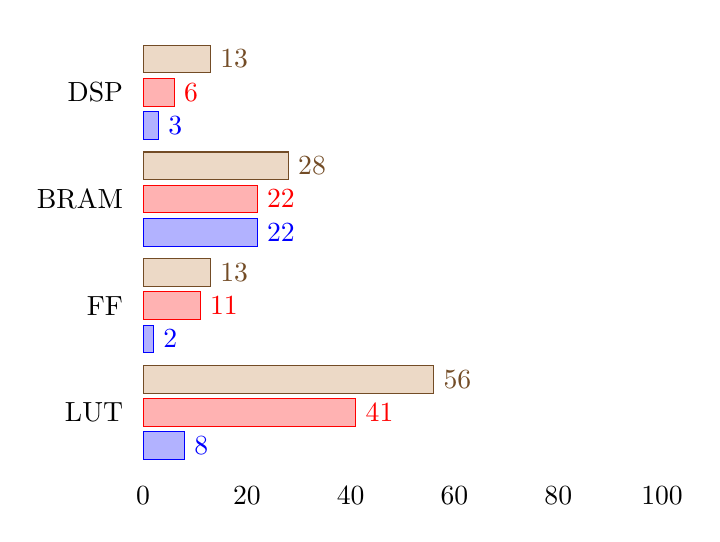
\begin{tikzpicture}
			\begin{axis}[	xbar,
						    y axis line style 	= { opacity = 0 },
						    % axis x line       	= none,
						    tickwidth         	= 0pt,
						    enlarge y limits  	= 0.2,
						    enlarge x limits  	= 0.02,
						    nodes near coords,
						    xmin 				= 0,
						    xmax 				= 100,
						    symbolic y coords 	= {LUT, FF, BRAM, DSP}]

	  			\addplot coordinates { (8,LUT)  	(2,FF)  	(22,BRAM) 	(3,DSP) };
	  			\addplot coordinates { (41,LUT)  	(11,FF) 	(22,BRAM) 	(6,DSP) };
	  			\addplot coordinates { (56,LUT)  	(13,FF) 	(28,BRAM) 	(13,DSP) };

	        \end{axis}
		\end{tikzpicture}
	\end{center}
	\caption{Ποσοστό αξιοποίησης πόρων συνάρτησης}
\end{figure}
\fi
Με βάση τα δεδομένα του προηγούμενου πίνακα γίνεται σαφές ότι η καλύτερη υλοποίηση είναι η τελευταία. Η τελική υλοποίηση προσφέρει ικανοποιητική συνολική επιτάχυνση και χαμηλή συχνότητα ρολογιού με μία ποσοστιαία αύξηση 900\% στην κατανάλωση των LUT. Έχει επιτευχθεί, επομένως ένας πολύ καλός συμβιβασμός μεταξύ απόδοσης και κατανάλωσης πόρων. Η συνολική κατανάλωση θα αυξηθεί βέβαια κατά τη διάρκεια του σχεδιασμού του πλήρους συστήματος στο Vivado IPI.

Μετά την επιτυχή προσομοίωση και εξαγωγή του υλικού στο HLS, σχεδιάζεται το πλήρες σύστημα στο Vivado όπως έχει περιγραφεί στο προηγούμενο κεφάλαιο. Το Vivado παράγει αναλυτική αναφορά σχετικά με τη τελική αξιοποίηση των διαθέσιμων πόρων.

Έχοντας ορίσει τη συχνότητα λειτουργίας του FPGA ίση με 100 MHz παρατηρούμε ότι για να ολοκληρωθεί η επεξεργασία της εικόνας εισόδου απαιτούνται 93278 κύκλοι ρολογιού. Επομένως, ο συνολικός χρόνος που απαιτείται για την επεξεργασία ενός frame είναι: $93278\times 10^{-8}= 0,00093278\ s = 0.93\ ms$.

Παρατηρείται επίσης, μία μείωση στο συνολικό αριθμό LUT που χρησιμοποιήθηκαν στο τελικό σχέδιο. Αυτή η διαφορά οφείλεται στο γεγονός οτι το HLS κάνει μία εκτίμηση της αξιοποίησης των πόρων καθώς και σε διάφορες βελτιστοποιήσεις που πραγματοποιοιεί το Vivado κατά τη διαδικασία της σύνθεσης.

\begin{table}[H]
\centering
\label{my-label}
\begin{tabular}{@{}c|c|c@{}}
\toprule
Πόροι & Αξιοποίηση & \multicolumn{1}{l}{Διαθέσιμοι} \\ \midrule
DSP & 48 & 220 \\
BRAM & 35 & 140 \\
FF & 16988 & 106400 \\
LUTRAM & 511 & 17400 \\
LUT & 14986 & 53200 \\ \bottomrule
\end{tabular}
\end{table}

\begin{figure}[H]
	\begin{center}
		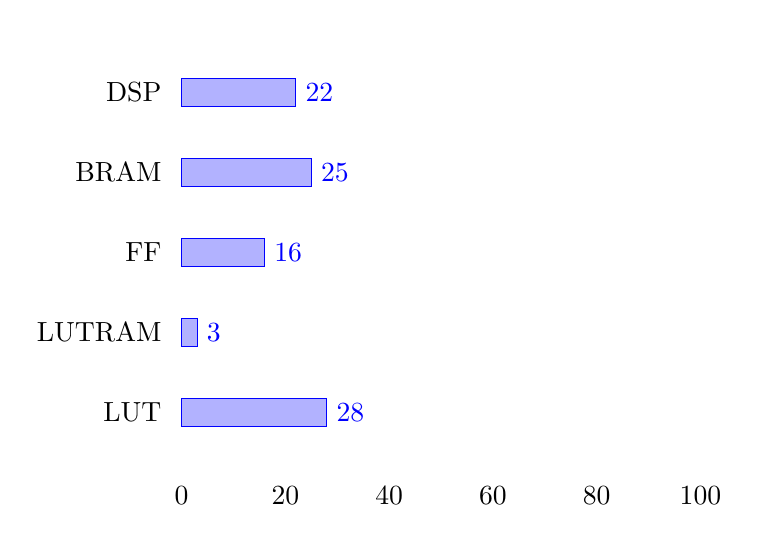
\begin{tikzpicture}
			\begin{axis}[	xbar,
						    y axis line style 	= { opacity = 0 },
						    % axis x line       	= none,
						    tickwidth         	= 0pt,
						    enlarge y limits  	= 0.2,
						    enlarge x limits  	= 0.02,
						    nodes near coords,
						    xmin 				= 0,
						    xmax 				= 100,
						    symbolic y coords 	= {LUT, LUTRAM, FF, BRAM, DSP}]

	  			\addplot coordinates { (28,LUT) (3,LUTRAM) (16,FF) (25,BRAM) (22,DSP) };
	        \end{axis}
		\end{tikzpicture}
	\end{center}
	\caption{Ποσοστό αξιοποίησης συνολικών πόρων}
\end{figure}
\noindent Στο ακόλουθο σχήμα φαίνεται η εκτίμηση της κατανάλωσης του συστήματος.

\begin{figure}[H]
   \centering
   \includegraphics[width=0.45\textwidth]{power}\\
   \caption{Εκτίμηση κατανάλωσης}
\end{figure}

\subsection{Αποτελέσματα επεξεργασίας}

Τελευταίο βήμα της εργασίας είναι η αξιολόγηση της σωστής λειτουργίας του αλγορίθμου επεξεργασίας ακμών που υλοποιήθηκε. Για το λόγο αυτό, επιλέχθηκαν τρεις διαφορετικές εικόνες που θα υποστούν επεξεργασία. Παράλληλα, θα επιλεχθούν τρείς διαφορετικές τιμές κατωφλίωσης, ώστε να επιλεχθεί εκείνη που παράγει τα βέλτιστα αποτελέσματα.
\begin{figure}[H]
\centering
\subcaptionbox{Είσοδος}%
  {\includegraphics[width=.22\linewidth]{lena}}
\subcaptionbox{$threshold = 40$}
  {\includegraphics[width=.22\linewidth]{lena40}}
\subcaptionbox{$threshold = 70$}
	{\includegraphics[width=.22\linewidth]{lena70}}
\subcaptionbox{$threshold = 120$}
	{\includegraphics[width=.22\linewidth]{lena120}}
\caption{Εικόνα \#1}
\end{figure}
\begin{figure}[H]
\centering
\subcaptionbox{Είσοδος}%
  {\includegraphics[width=.22\linewidth]{stop}}
\subcaptionbox{$threshold = 40$}
  {\includegraphics[width=.22\linewidth]{stop40}}
\subcaptionbox{$threshold = 70$}
	{\includegraphics[width=.22\linewidth]{stop70}}
\subcaptionbox{$threshold = 120$}
	{\includegraphics[width=.22\linewidth]{stop120}}
\caption{Εικόνα \#2}
\end{figure}
\begin{figure}[H]
\centering
\subcaptionbox{Είσοδος}%
  {\includegraphics[width=.22\linewidth]{a}}
\subcaptionbox{$threshold = 40$}
  {\includegraphics[width=.22\linewidth]{flower40}}
\subcaptionbox{$threshold = 70$}
	{\includegraphics[width=.22\linewidth]{flower70}}
\subcaptionbox{$threshold = 120$}
	{\includegraphics[width=.22\linewidth]{flower120}}
\caption{Εικόνα \#3}
\end{figure}

Παρατηρούμε ότι ο αλγόριθμος μας παράγει σωστά αποτελέσματα με καλά αναγνωρισμένες ακμές. Επίσης, είναι εμφανές ότι η τιμή του κατωφλίου που δίνει τα καλύτερα αποτελέσματα διαφέρει απο εικόνα σε εικόνα. Επομένως, η σωστή τιμή επιλέγεται με τη μέθοδο "trial \& error". H τιμή $threshold = 40 $ δίνει όμως τα καλύτερα αποτελέσματα σε σταθερή βάση.
